\subsection{HTB02 - Time}

    \subsubsection{Escaneo}
        \large{Como primera etapa de la Prueba de Penetración realizamos un escaneo de puertos abiertos en la máquina víctima con la herramienta "Nmap", donde se encuentran dos de ellos, el 22 con el servicio SSH y el 80 con un servidor web Apache.}
        \par
        \begin{figure}[H]
            \centering
            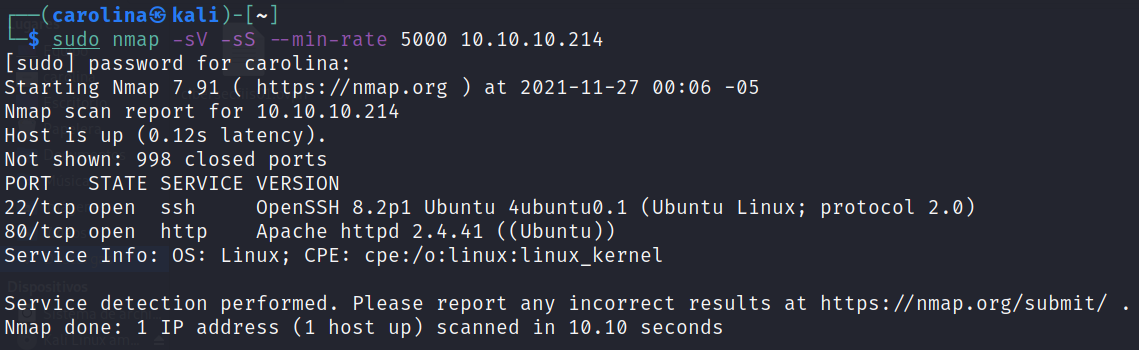
\includegraphics[width=0.99\textwidth]{imagenes/time/01_nmap_time.png} 
            \caption{Escaneo de puertos Time} 
        \end{figure}

    \subsubsection{Análisis de Vulnerabilidades}

    \subsubsection{Explotación}

    \subsubsection{Escalamiento de Privilegios}

    \subsubsection{Post-Explotación}

    \subsubsection{Recomendaciones de Mitigación}
